\newpage
\hypertarget{stringRep tex}{}
\subsection{Implementing stringRep}
\texHeader

\vspace{0.5cm}

\begin{itemize}
  
\item[$\blacktriangleright$] Closely following Fig.~\ref{fig:goal_stringRep}, create a nested \texttt{forEach} loop in \texttt{Box.toString()}.
Don't worry about invoking \texttt{addToStringRep} yet -- just make sure you return the \texttt{this.stringRep} attribute. It should resemble
Fig.~\ref{fig:emptyLoops}.

\begin{figure}[htp]
\begin{center}
  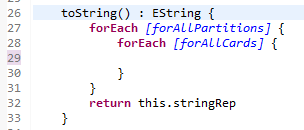
\includegraphics[width=0.5\textwidth]{eclipse_toStringNestedLoops}
  \caption{Control flow for \texttt{toString}}
  \label{fig:emptyLoops}
\end{center}
\end{figure}

\item[$\blacktriangleright$] Now, in order to use \texttt{addToStringRep}, we need create another \emph{statement node}. Inside the second loop, write:
\syntax{<@this.addToStringRepCard(card)>} 
The correct \texttt{card} parameter will be matched by the \texttt{ForAllCards} pattern; We'll establish this next.

\vspace{0.5cm}

\item[$\blacktriangleright$] The completed \texttt{toString} activity should now resemble Fig.~\ref{fig:toStringFlow}.

\vspace{0.5cm}

\begin{figure}[htp]
\begin{center}
  \includegraphics[width=0.6\textwidth]{eclipse_boxtoStringFlow}
  \caption{Using a \emph{statement node} as part of the control flow}
  \label{fig:toStringFlow}
\end{center}
\end{figure}

\item[$\blacktriangleright$] Don't forget that the aim of the activity is to access every item in \texttt{Box}. The control flow finishes when the helper
method is able to called for all existing cards. This means the \texttt{forAllPartitions} and \texttt{forAllCards} patterns only need to match their
namesake's object variable to ensure that all cards in all partitions are found.

\clearpage

\item[$\blacktriangleright$] Complete each pattern as depicted in Fig.~\ref{fig:toStringPatterns}. The \texttt{partition} in \texttt{forAllCards} is bound to
the one matched in the current (first) loop iteration, but \texttt{card} is \emph{not} bound as it must be newly matched each time.

\vspace{0.5cm}

\begin{figure}[htp]
\begin{center}
  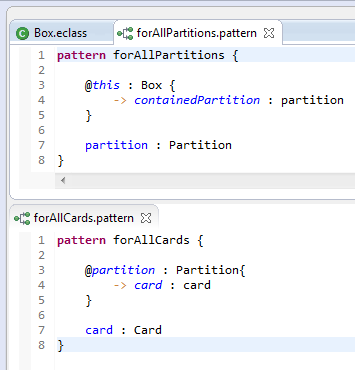
\includegraphics[width=0.6\textwidth]{eclipse_toStringPatterns}
  \caption{Box traversal patterns}
  \label{fig:toStringPatterns}
\end{center}
\end{figure}

\vspace{0.5cm}

\item[$\blacktriangleright$] As crazy at it may seem, that's it!  To see how this SDM is represented visually, check out Fig.~\ref{fig:sdm_tostring_5}.

\end{itemize}
